

\section{Code-Quality-Benchmark mit anderen Ruby-Projekten}

Um die Ergebnisse besser einordnen zu können, vergleichen wir die Ergebnisse aus den Code-Quality-Benchmark mit vergangenen Ruby\index{Ruby}-Projekten in der pludoni GmbH und mit bekannten Ruby/Rails\index{Ruby-on-Rails}-OpenSource Applikationen und Bibliotheken.

Eine vollständige Metrik wie oben an IT-Jobs\index{IT-Jobs-Projekt}, war in vielen Fällen nicht möglich, da die Testwerkzeuge in vielen Fällen Inkompatibilitäten mit neueren Rubyversionen haben. Wir beschränken uns deshalb auf eine exemplarische Überblicksmetrik, bestehend aus:

\begin{description}
 \item[LOC] Anzahl der Quellcodezeilen, gemessen durch das Rails\index{Ruby-on-Rails}-Kommando "`rake stats"'. 
 \item[LOT] Anzahl der Quellcodezeilen aller Tests, gemessen durch das Rails-Kommando "`rake stats"'. 
 \item[LOT/TOC] Verhältnis aus Testzeilen und Quellcodezeilen
 \item[AVGCmplx] Durchschnittliche Komplexität aller Klassen, gemessen durch \textbf{Flog}\footnote{\url{https://github.com/seattlerb/flog}}. Flog besitzt ein eigenes Maß für Code-Komplexität. Es vergibt für jede Zuweisungen, Verzweigungen und Funktionsaufrufe unterschiedlich viele Punkte und bildet so eine Summe per Funktion oder per Klasse. Dabei vergibt Flog besonders viele Punkte für schwer nachzuvollziehende Funktionsaufrufe, wie z.B. "`eval(string)"', welches einen String als Ruby\index{Ruby}-Code auswertet.
 \item[H5Cmplx] Komplexität der 5\% komplexesten Klassen, nach Flog
 \item[DSmell] Anzahl der Code-Smells nach Roodi. Beinhaltet u.a.: hohe Cyclomatische Komplexität in einer Methode (min. 4), lange Methoden, lange Parameterlisten, u.v.m.\footnote{\url{http://roodi.rubyforge.org/files/README_txt.html}}
 \item[DSmell/KLOC] Anzahl der Code-Smells nach Roodi pro tausend Codezeilen
 \item[CSmell] Anzahl der Code-Smells nach Reek. Diese beinhalten: Geringe Kohäsion, Duplikation, Control-Couple, Unkommunikativer Name von Methoden/Variablen/Parameter, verschachtelte Iteratoren, u.v.m  \footnote{\url{https://github.com/kevinrutherford/reek/wiki/Code-Smells}}
 \item[CSmell/KLOC] Anzahl der Code-Smells nach Reek pro tausend Codezeilen
\end{description}







\subsection{Vergleich von IT-Jobs mit eigenen Projekten}

Bisherige Projekte der pludoni GmbH und des Autors basierend auf Ruby\index{Ruby}/ Ruby on Rails\index{Ruby-on-Rails}
\begin{description}
 \item[feedimport] Ist die fertiggestellte Bibliothek, die im Rahmen der Entwicklung von IT-Jobs\index{IT-Jobs-Projekt} ausgelagert wurde, um den Community-Portalen bereits jetzt zur Verfügung zu stehen. Die Grundzüge wurden in Abschnitt \ref{sec:awmock} vorgestellt.
 \item[feedmerger] Eine Rails\index{Ruby-on-Rails}-Anwendung\footnote{ Als OpenSource unter \url{https://github.com/zealot128/WenShanWenHai} zu finden.} zur Verwalten, Cachen, Filtern und Zusammenfügen von RSS und Atom-Feeds.
 \item[pludonidb] Ist eine auf ActiveRecord\index{ActiveRecord} basierende Bibliothek zur Anbindung der Datenbanken der Communityportale an Ruby-Skripte. Beinhaltet außerdem weitere Hilfsfunktionen für Berechnung von Tag-Wolken, Häufigkeiten u.ä.
 \item[backlinks] Backlink und SEO-Success-Control ist eine Rails-2.3 Anwendung, zum Messen der sogenannten Backlinks\footnote{Backlinks sind Links anderer Webseiten auf die eigenen. In den Communityportalen sind die Mitglieder vertraglich verpflichtet, einen Backlink auf die Communityportale anzulegen.} der Communitymitglieder und der Platzierung für relevante Sucheingaben in den großen Suchmaschinen (konkret: Welchen Platz hatte ein Communityportal an einem bestimmten Tag für "`it jobs dresden"', usw.). Details dazu sind im Praktikumsbericht des Autors zu finden. %TODO Verweis auf meinen Praktikumsbericht
 
 \item[SiteAnalyzer (SAnalyzer)] ist ein Werkzeuge zur Analyse von kompletten Websites/Webdomains, mit dem Ziel tote Links zu finden, alle Seiten auf HTML-Gültigkeit zu prüfen und insgesamt die Link-Architektur zu analysieren\footnote{Auch dieses Projekt ist als OpenSource verfügbar: \url{https://github.com/zealot128/Site-Structure-Analyzer}}. 
\end{description}


\begin{table}[hbp]
 \caption{Vergleich von IT-jobs mit anderen Ruby Projekten des Autors/der pludoni GmbH}\label{table:cmpmy}
 \begin{center}
 
\begin{tabular}{|l|l|l|l|l|l|l|}
\hline\rowcolor{tableheadcolor}

Projekt&ItJobs&Backlinks&Feedmerger&SAnalyzer&Feedimport&PludoniDb\\
\hline
Technologie&Rails3&Rails2&Rails3&Rails3&Ruby&Ruby\\
\hline
Testverfahren&TDD&manuell&manuell&manuell&TDD&manuell\\
\hline
LOC&1570&1884&724&214&571&1933\\
\hline
LOT&1750&75&137&0&865&126\\
\hline
LOT/LOC&1.11&0.04&0.19&0.00&1.51&0.07\\
\hline
AVGCmplx&8.00&19.90&10.50&14.80&16.80&13.70\\
\hline
H5Cmplx&43.80&70.60&26.90&39.70&25.10&113.20\\
\hline
DSemll&11&69&11&11&8&25\\
\hline
DSmell/KLOC&7.00&36.60&15.20&51.40&14.00&12.90\\
\hline
CSmell&53&152&52&13&28&113\\
\hline
CSmell/KLOC&33.80&80.70&71.80&60.70&49.00&58.50\\
\hline
\end{tabular}
\end{center}

\end{table}


\subsection{Vergleich von IT-Jobs mit anderen Rails-Projekten}
Weiterhin wird das Projekt mit folgenden beliebten Webprojekten, welche ebenfalls auf Ruby on Rails\index{Ruby-on-Rails} basieren, verglichen:
\begin{description}
\item[lpp] Linkpartnerprogramm ist eine Studenteninitiative der TU Dresden, um ausländische Studenten mit deutschen Sprach- und Lernpartnern zusammenzubringen. Dazu wurde 2008 von einem Studententeam im Rahmen einer Semesterarbeit eine Rails\index{Ruby-on-Rails}-Webanwendung geschrieben. Der Autor dieser Arbeit war zwar nicht an der Entwicklung beteiligt, übernahm aber die Pflege und Weiterentwicklung selbiger.
 \item[diaspora] Ist ein verteiltes soziales Netzwerk. \\
 Code: \url{https://github.com/diaspora/diaspora}
 \item[bucketwise (bucket)] ist ein web-basierter persönlicher Finanzmanager mit Budgetierung nach dem Briefumschlagsystem\\
 Code: \url{https://github.com/jamis/bucketwise}
 \item[chiliproject (chilli)] Ist ein Fork\footnote{In der (Open-Source) Software-Entwicklung ist ein Fork eine legale Kopie eines bestehendes Software-Produktes, um von nun an eine unabhängige Entwicklung zu betreiben} des sehr beliebten Bugtrackers Redmine\footnote{https://github.com/edavis10/redmine}. Statt des originalen Redmines wurde dieser Fork genommen, da er eine neuere Codebasis hat\\
 Code: \url{https://github.com/chiliproject/chiliproject}
 \item[railscast (rCasts)] Ist der Code der Website \url{http://www.railscasts.com}, in welche allwöchentlich ein Screencast zum Thema Ruby und Rails veröffentlich wird (bis dato 283 Episoden).\\
 Code: \url{https://github.com/ryanb/railscasts} 
 \item[ActiveSupport [aSupport]] Beinhaltet Hilfsklassen und Erweiterungen der Ruby-Standardbibliothek und ist Kernbestandteil von Ruby on Rails \\
 Code: \url{https://github.com/rails/rails.git}
 \item[ActionPack (aPack)]  ist ein Framework um Anfragen und Antworten eines Webservers zu verarbeiten und ist ein weiterer Kernbestandteil von Rails.\\
 Code: \url{https://github.com/rails/rails.git}
\end{description}

Die Auswahl erfolgt z.T. sehr willkürlich. Als Ansatzpunkt diente die Liste der beliebtesten Rails\index{Ruby-on-Rails}-Projekte, die auf Github gehostet sind. Weiterhin wurde ActiveSupport und ActionPack ausgewählt, um die Code-Qualität von Rails selbst mit zu beurteilen.

\begin{table}[hbp]
 \caption{Vergleich von IT-jobs mit Ruby/Rails Projekten aus der Community}\label{table:cmpother}
 \begin{tabular}{|p{1.8cm}|l|l|l|l|l|l|l|l|}
\hline \rowcolor{tableheadcolor}
 Projekt&itjobs&bucket&lpp&chili&aPack&aSupport&diaspora&rCasts\\
\hline
Technol.&Rails3&Rails2&Rails1&Rails2&Rails3&Rails3&Rails3&Rails3\\
\hline
LOC&1570&1979&7116&21201&12995&9407&7466&653\\
\hline
LOT&1750&1684&1557&20127&32570&13590&10072&748\\
\hline
LOT/LOC&1.11&0.85&0.22&0.95&2.51&1.44&1.35&1.15\\
\hline
AVGCmplx&8.00&12.80&17.10&19.10&11.10&10.90&13.10&11.00\\
\hline
H5Cmplx&43.80&32.20&181.80&84.40&64.00&47.90&54.00&34.60\\
\hline
DSmell&11&37&250&651&370&166&99&2\\
\hline
DSmell\newline~/KLOC&7.00&18.70&35.10&30.70&28.50&17.60&13.30&3.10\\
\hline
CSmell&53&129&386&1535&982&291&324&42\\
\hline
CSmell\newline~/KLOC&33.80&65.20&54.20&72.40&75.60&30.90&43.40&64.30\\
\hline
\end{tabular}
\end{table}

\subsection{Auswertung und Visualisierung}
In den Abbildungen \ref{fig:cpm-loclot}, \ref{fig:cpm-complex} und \ref{fig:cpm-smells} werden die gesammelten Ergebnisse für alle genannten Projekte visualisiert. Der obere Teil jeder Abbildung enthält die externen Projekte, der untere alle Projekte der pludoni GmbH.
\begin{figure}[htbp]
 \centering
 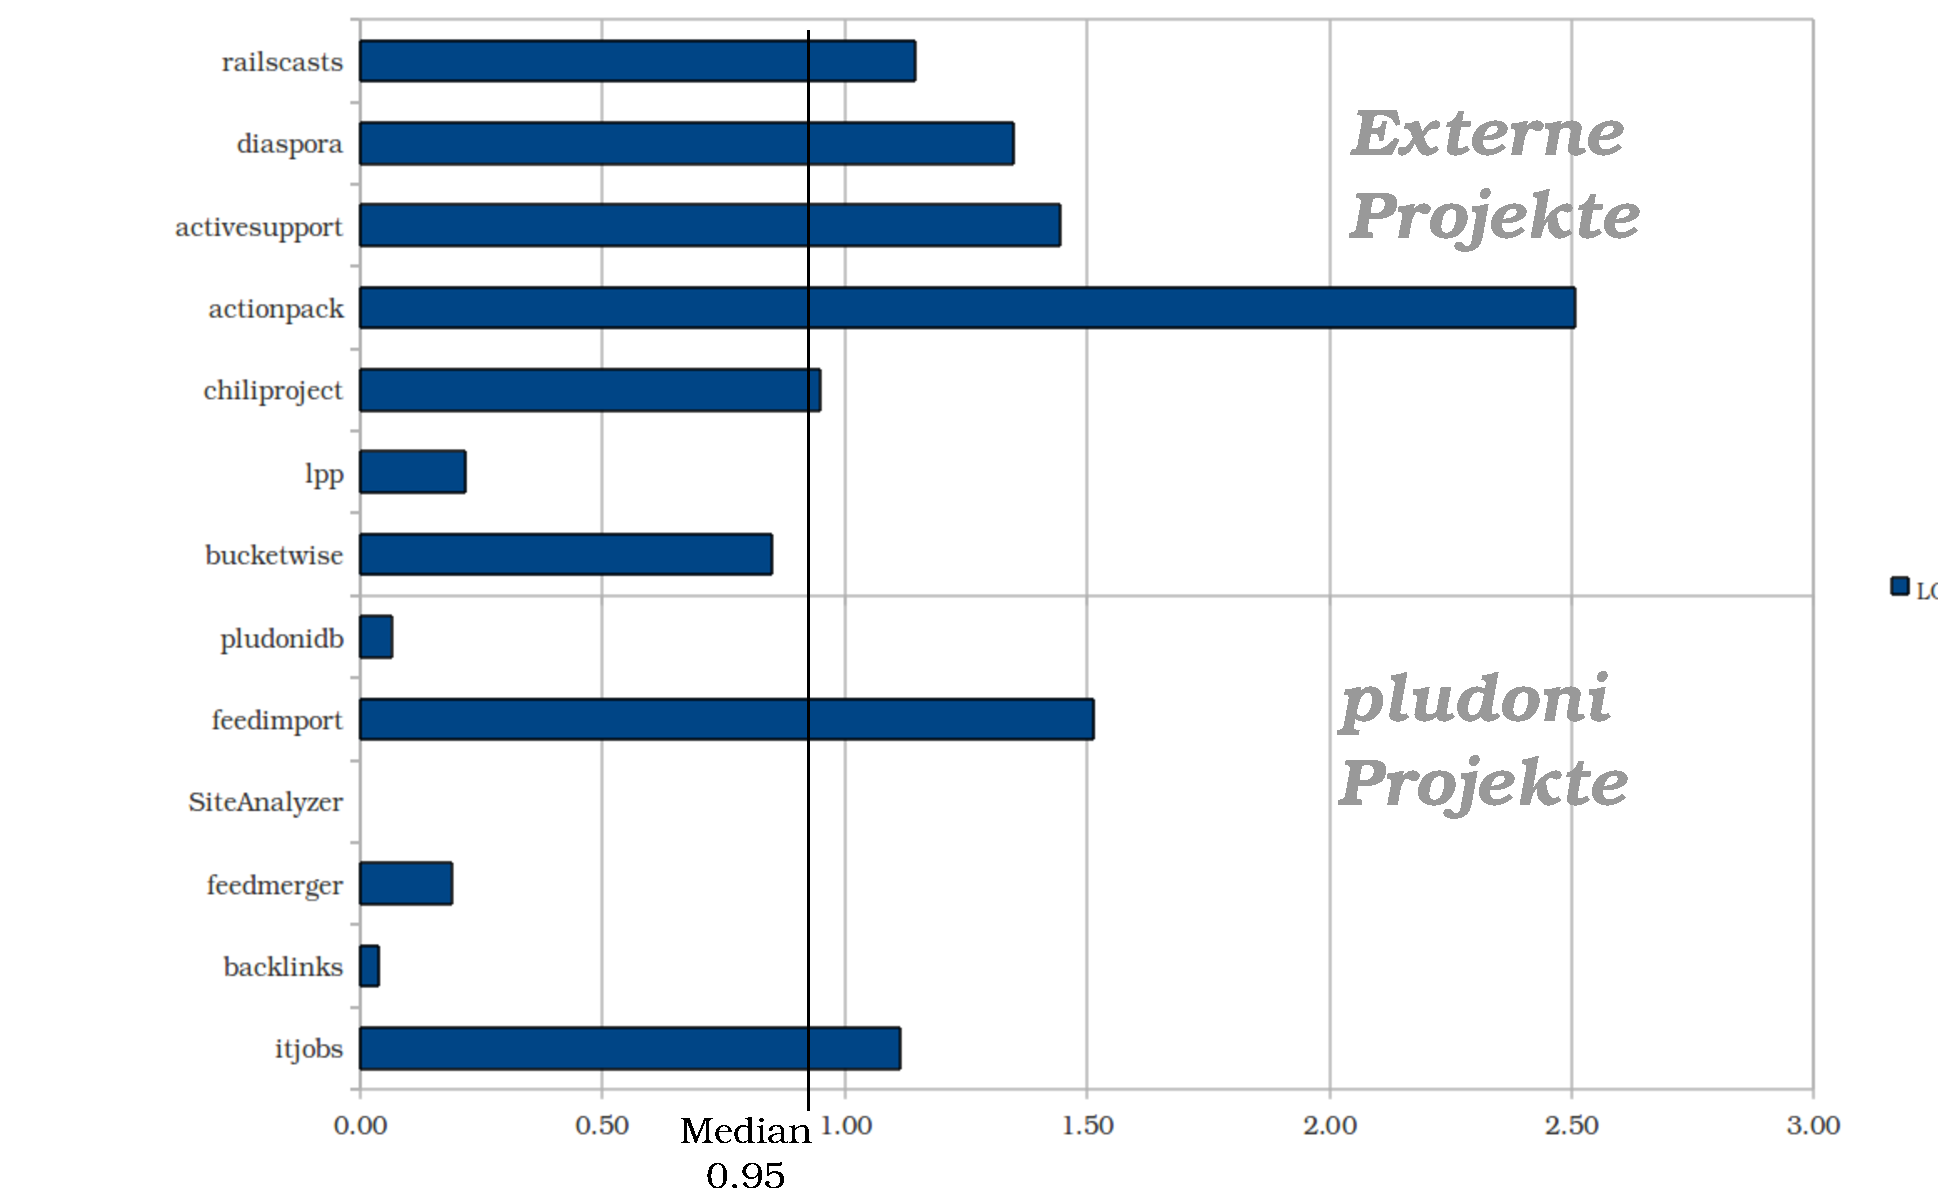
\includegraphics[width=\linewidth]{./diagrams/cpm-lotloc.pdf}
 % cpm-lotloc.pdf: 930x574 pixel, 72dpi, 32.81x20.25 cm, bb=0 0 930 574
 \caption{Vergleich des Verhältnisses aus Anzahl Testcodezeilen / Anzahl Codezeilen}
 \label{fig:cpm-loclot}
\end{figure}

Abbildung \ref{fig:cpm-loclot} zeigt das Verhältnis aus Testcode zu Programmcode. Der Median über alle Projekte ist 0.95. Ausreißer sind hierbei vier der internen Projekte pludonidb, SiteAnalyzer, feedmerger und backlinks, die wenig bis gar keine automatisierten  Tests besitzen. Als Gegenbeispiel sei ActionPack zu nennen, dass über 2.5x soviel Testcodezeilen wie Programmcode verfügt. Gegenüber den bisherigen Projekten in der pludoni GmbH kann man anhand der Projekte Feedimport und IT-Jobs\index{IT-Jobs-Projekt}, die im Rahmen dieser Diplomarbeiten enstanden, sehen, dass die bloße Anzahl an Tests stark zugenommen hat. Beide Projekte wurden mittels TDD\index{TDD} entwickelt. Gegenüber dem Feedimport verfügt IT-Jobs aber über mehr Code, der durch das Framework bereits zur Verfügung gestellt wird, während der Feedimport eine weitestgehend eigene Objekthierarchie besitzt und damit auch mehr Tests bedurfte.

\begin{figure}[htbp]
 \centering
 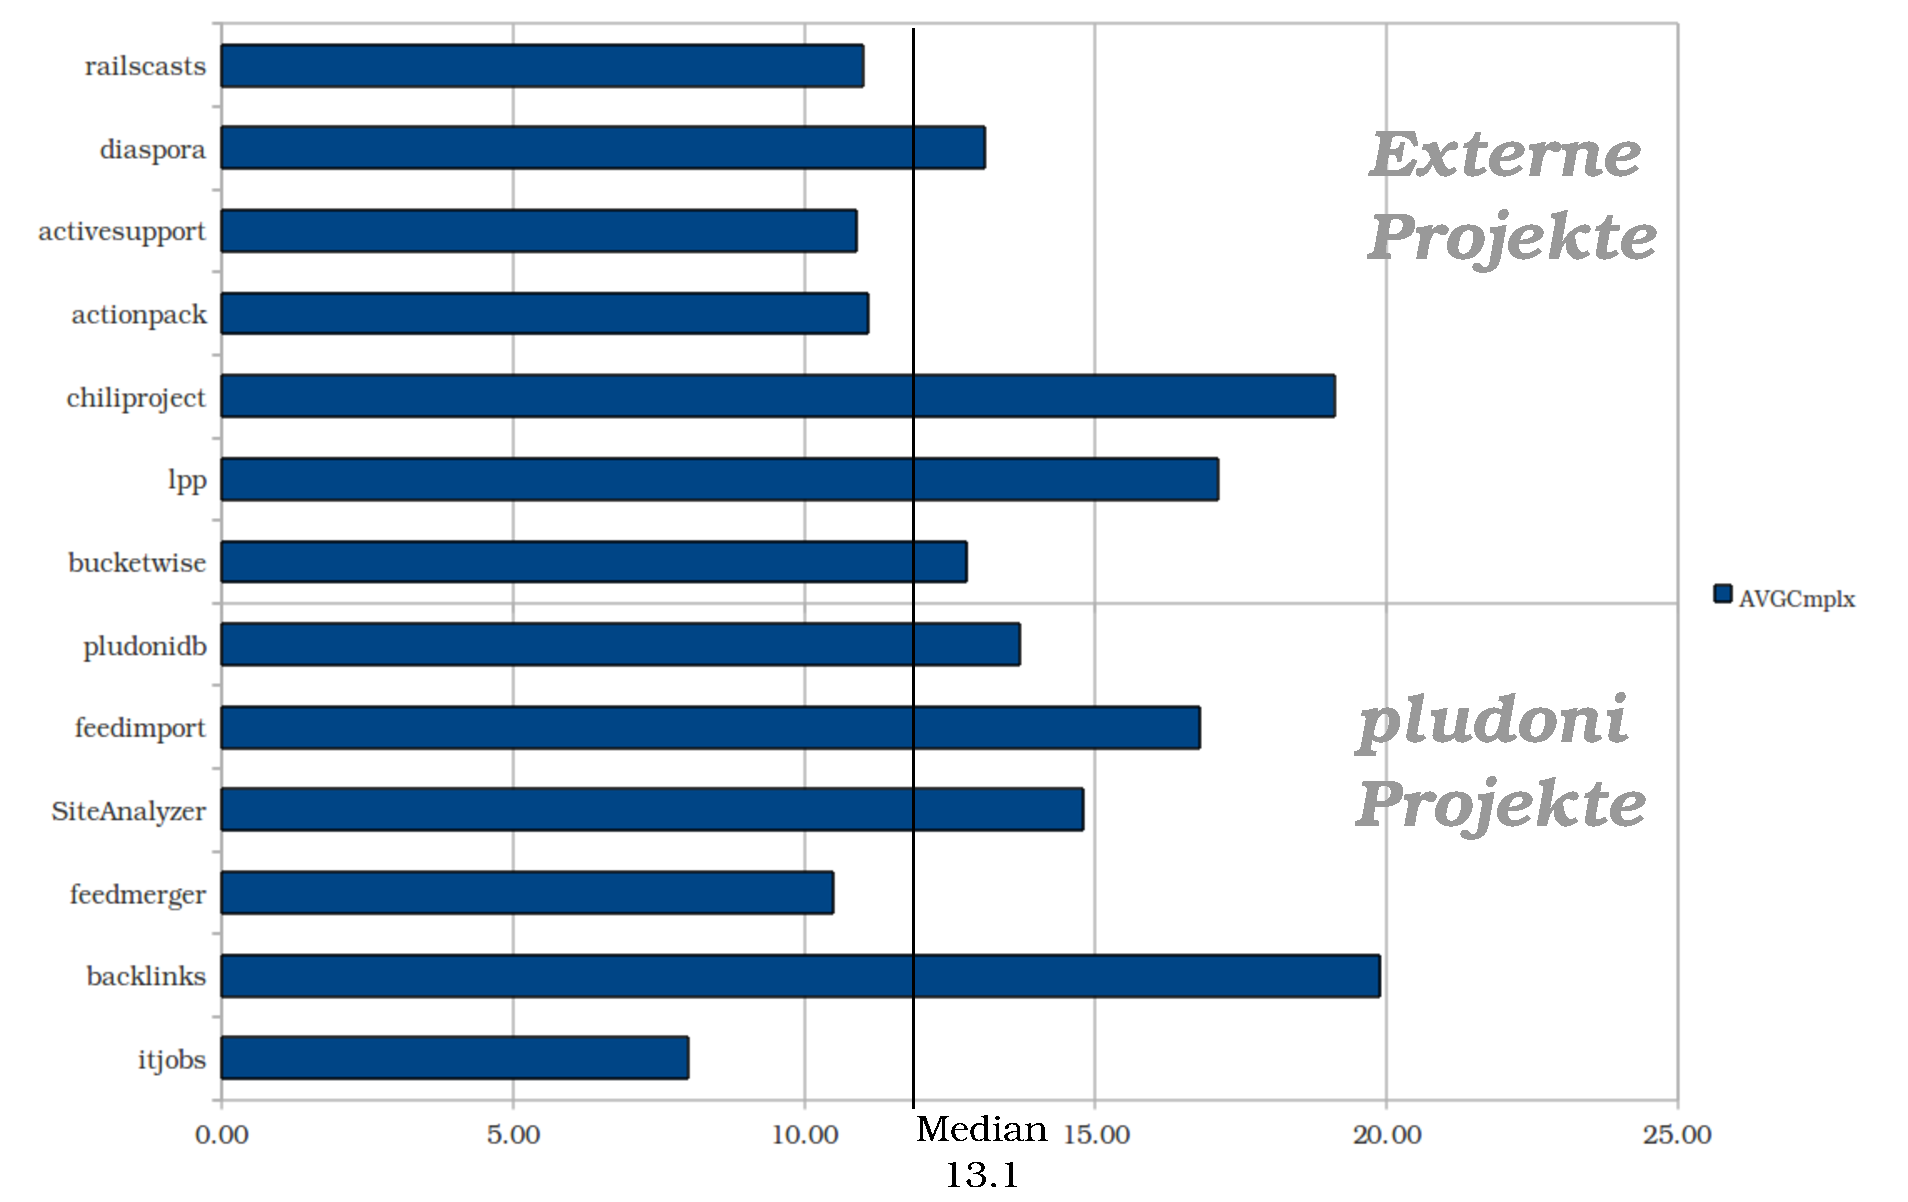
\includegraphics[width=\linewidth]{./diagrams/cmp-complex.pdf}
 % cpm-lotloc.pdf: 930x574 pixel, 72dpi, 32.81x20.25 cm, bb=0 0 930 574
 \caption{Vergleich der durchschnittlichen Komplexität}
 \label{fig:cpm-complex}
\end{figure}
In Abbildung \ref{fig:cpm-complex} wurde die durchschnittliche Komplexität nach dem Flog-Verfahren gegenübergestellt. Der Median war hier 13,1. Unter den eigenen Projekten sind hier Backlinks und der Feedimport die komplexesten Projekte. IT-Jobs\index{IT-Jobs-Projekt} und Feedmerger, die beide Rails-Projekte sind, haben dagegeben eine geringere Code-Komplexität. Die Ursache ist hierbei, dass während der Entwicklung von IT-Jobs ständig die Code-Qualität durch die Metriken gemessen wurde und im Falle von Ausreißern gegengesteuert wurde. Bei dem Feedimport, der zwar durch TDD\index{TDD} entwickelt wurde, wurde eine solche Analyse erst am Ende der Entwicklung durchgeführt. Für uns ist das ein Indiz, dass das Nutzen einer Testgetriebenen Entwicklung kein alleiniger Garant für eine gute Code-Qualität ist.\\
Bei den externen Projekten war der Bugtracker-Anwendung Chiliproject/Redmine die komplexeste Anwendung, dicht gefolgt von der Sprachpartnervermittlung Linkpartnerprogramm. Gerade wenn man das Verhältnis aus Testcode zu Programmcode mit einbezieht, kann man eine Tendenz ableiten: Beide Projekte haben gegenüber den anderen externen eine relativ geringe Anzahl an Testcode und beide haben eine relativ hohe Komplexität.

\begin{figure}[htbp]
 \centering
 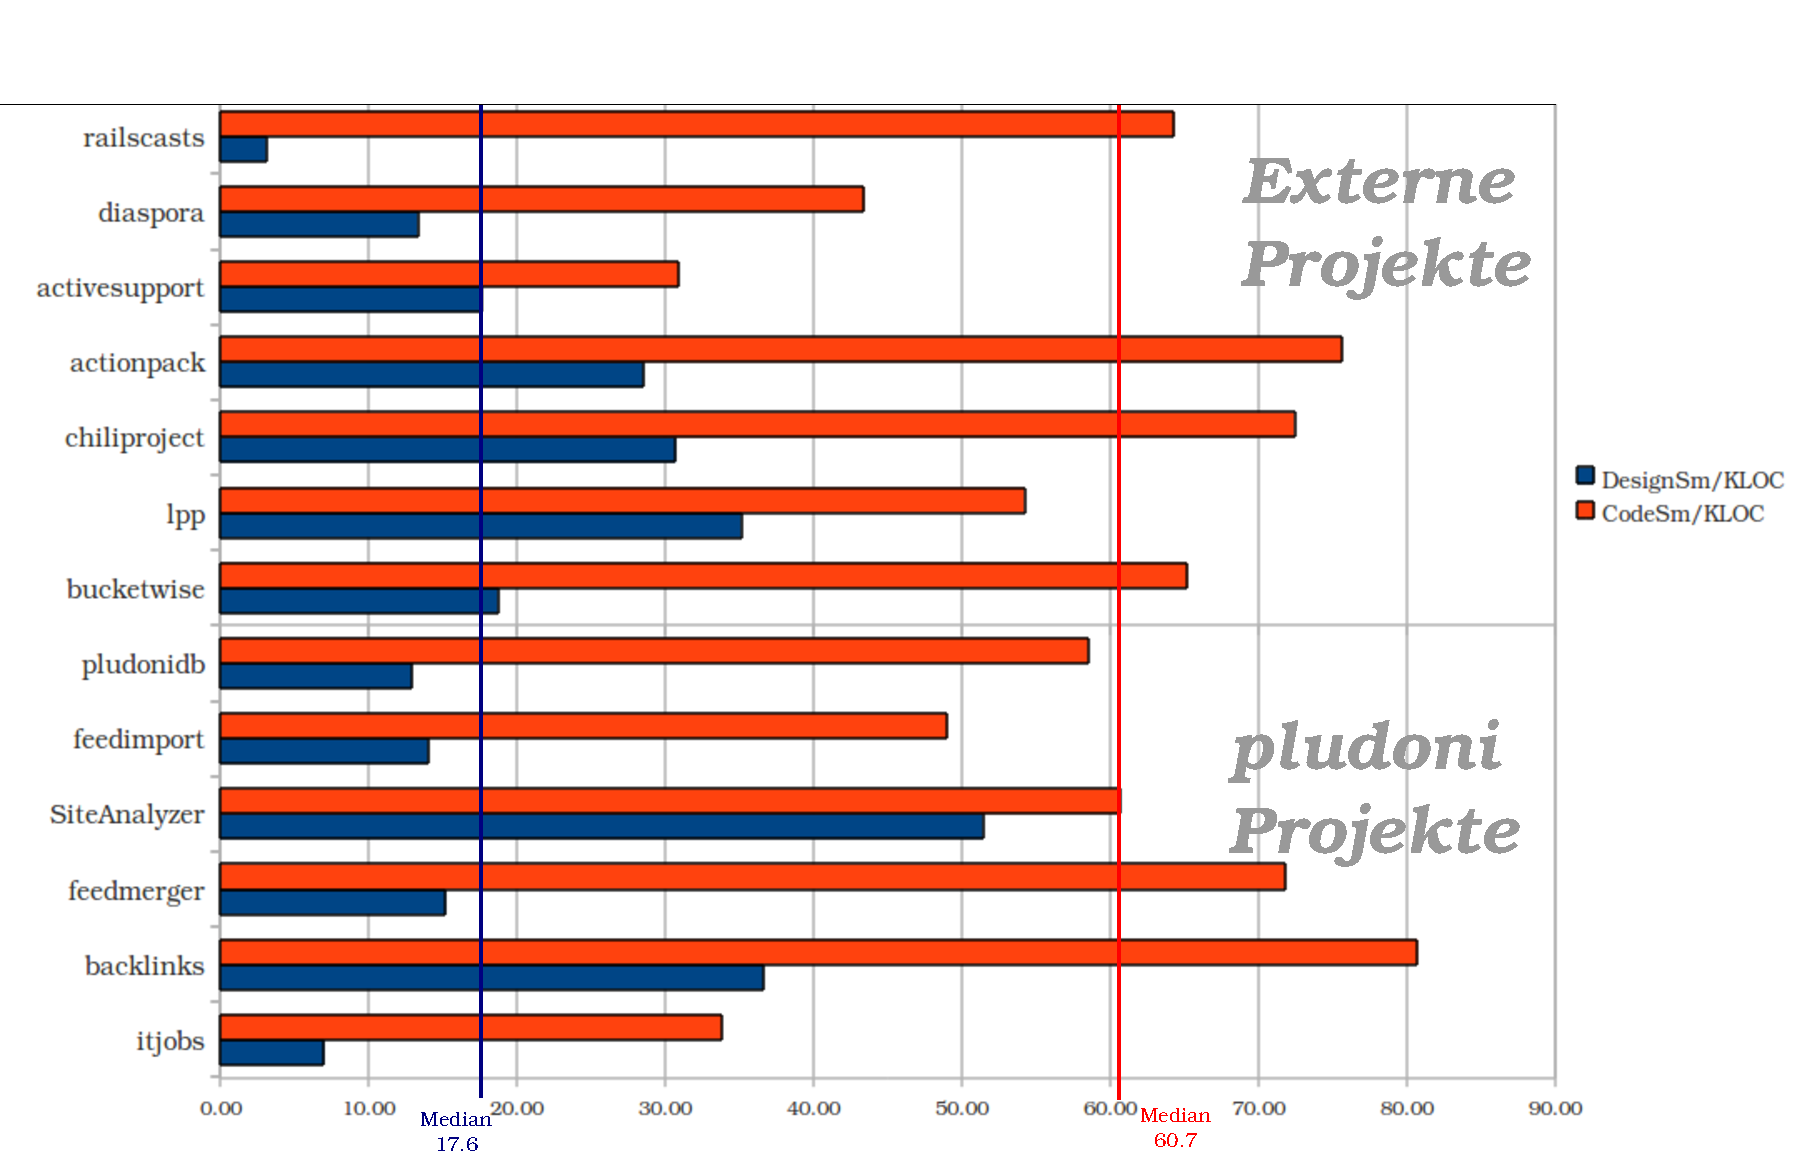
\includegraphics[width=\linewidth]{./diagrams/cpm-smells.pdf}
 % cpm-lotloc.pdf: 930x574 pixel, 72dpi, 32.81x20.25 cm, bb=0 0 930 574
 \caption{Vergleich der Anzahl Smells pro KLOC}
 \label{fig:cpm-smells}
\end{figure}
Die Abbildung \ref{fig:cpm-smells} zeigt zwei verschiedene Arten von Smell\index{Code-Smell}s: Einerseits durch Reek gemessen (Rot) und andererseits durch Roodi gemessen (Blau). Zu bemerken sei, dass IT-Jobs\index{IT-Jobs-Projekt} eine deutlich geringere Code-Smell-Dichte (1/2 Median) besitzt. Auch der Feedimport ist noch im Rahmen und leicht unter dem Schnitt. Dagegen hat das interne Projekt Backlinks die höchste Dichte an Code-Smells. Interessanterweise hat dieses Projekt auch so gut wie gar keine automatisierten Tests, was eine nachträgliche Refaktorisierung\index{Refaktorisierung} sehr erschwert. Für das Projekt Feedimport existiert allerdings eine gute Testabdeckung\index{Test!Testabdeckung} und so ließen sich leicht weitere Refaktorisierungen durchführen, sollte das gewünscht sein. \\
Actionpack verfügt unter den externen Projekten die höchste Smell\index{Code-Smell}-Dichte, trotz der großen Menge an Tests und der relativ geringen Komplexität. Da Actionpack auf das umfangreichste Projekt unter den untersuchten ist, wäre hier ein guter Ansatzpunkt für weitere Untersuchungen in der Sinnhaftigkeit gewissen Code-Smells. Die mit Abstand größte Code-Smell hierbei war Geringe Kohäsion bzw. starke Kopplung unter den Klassen. Eventuell lassen sich einige der Smells bei großen Modulen nicht vermeiden, da diese zwangsweise untereinander gekoppelt sein müssen.



Für statistisch signifikante Ergebnisse reichen die hier präsentierten Daten nicht aus, stattdessen sollte nur eine Tendenz untersucht werden. Insbesondere der Vergleich mit den internen Projekten hinsichtlich Code-Qualität. Das Gefühl der Programmierer, das z.B. das Projekt Backlinks eine relativ schlechte Codebasis verfügt, wurde durch die hier gezeigten Metriken bestätigt. Der aktuelle Stand von IT-Jobs\index{IT-Jobs-Projekt} dagegen lässt eine gute Ausgangsbasis für eine Weiterentwicklung vermuten.


